\chapter{Recursion}

\section{Tower of Hanoi}

\subsection*{Recursive Formula}
Let $T(n)$ denote the minimum number of moves required to solve the Tower of Hanoi problem with $n$ disks.

\begin{tabular}{@{}lccc}
   Recurrence relation
   & Single Tower of Hanoi
   & Double Tower of Hanoi
   & Triple Tower of Hanoi \\
   &: \ $T_n = 2T_{n-1} + 1$
   &: \ $T_n = 2T_{n-1} + 2$
   &: \ $T_n = 2T_{n-1} + 3$\\[1em]
   
   Close Form
   & Single Tower of Hanoi
   & Double Tower of Hanoi
   & Triple Tower of Hanoi \\
   &: \ $T_n = 1\left(2^n - 1\right)$
   &: \ $T_n = 2\left(2^n - 1\right)$
   &: \ $T_n = 3\left(2^n - 1\right)$
\end{tabular}


\vspace{1em}
\textbf{Find the number moves required to move 8 disks}
\begin{center}
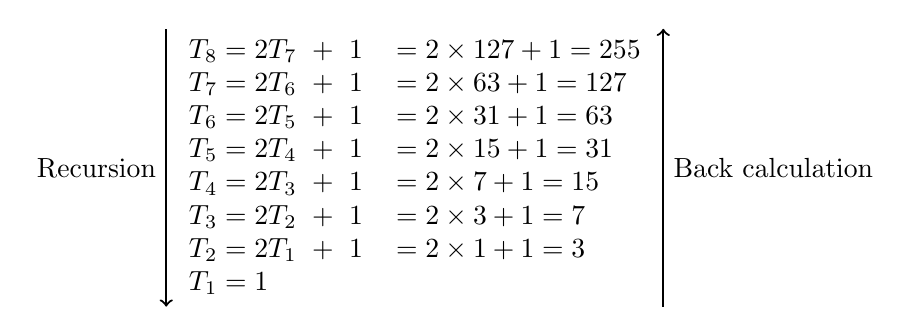
\begin{tikzpicture}
   \node[inner sep=2pt] (t) {
      \begin{tabular}{ll}
      $T_8 = 2T_7 \ + \ 1$ & $= 2\times 127 + 1 = 255$ \\
      $T_7 = 2T_6 \ + \ 1$ & $= 2\times 63 + 1 = 127$ \\
      $T_6 = 2T_5 \ + \ 1$ & $= 2\times 31 + 1 = 63$ \\
      $T_5 = 2T_4 \ + \ 1$ & $= 2\times 15 + 1 = 31$ \\
      $T_4 = 2T_3 \ + \ 1$ & $= 2\times 7 + 1 = 15$ \\
      $T_3 = 2T_2 \ + \ 1$ & $= 2\times 3 + 1 = 7$ \\
      $T_2 = 2T_1 \ + \ 1$ & $= 2\times 1 + 1 = 3$ \\
      $T_1 = 1$ \\
      \end{tabular}
   };
   
   \draw[<-, thick] (t.south west) -- (t.north west) node[midway,left] {Recursion};
   \draw[->, thick] (t.south east) -- (t.north east) node[midway,right] {Back calculation};
\end{tikzpicture}
\end{center}

For $n = 8$ disks, $T(8) = 2^8 - 1 = 256 - 1 = 255$

\pagebreak
\begin{figure}[h]
   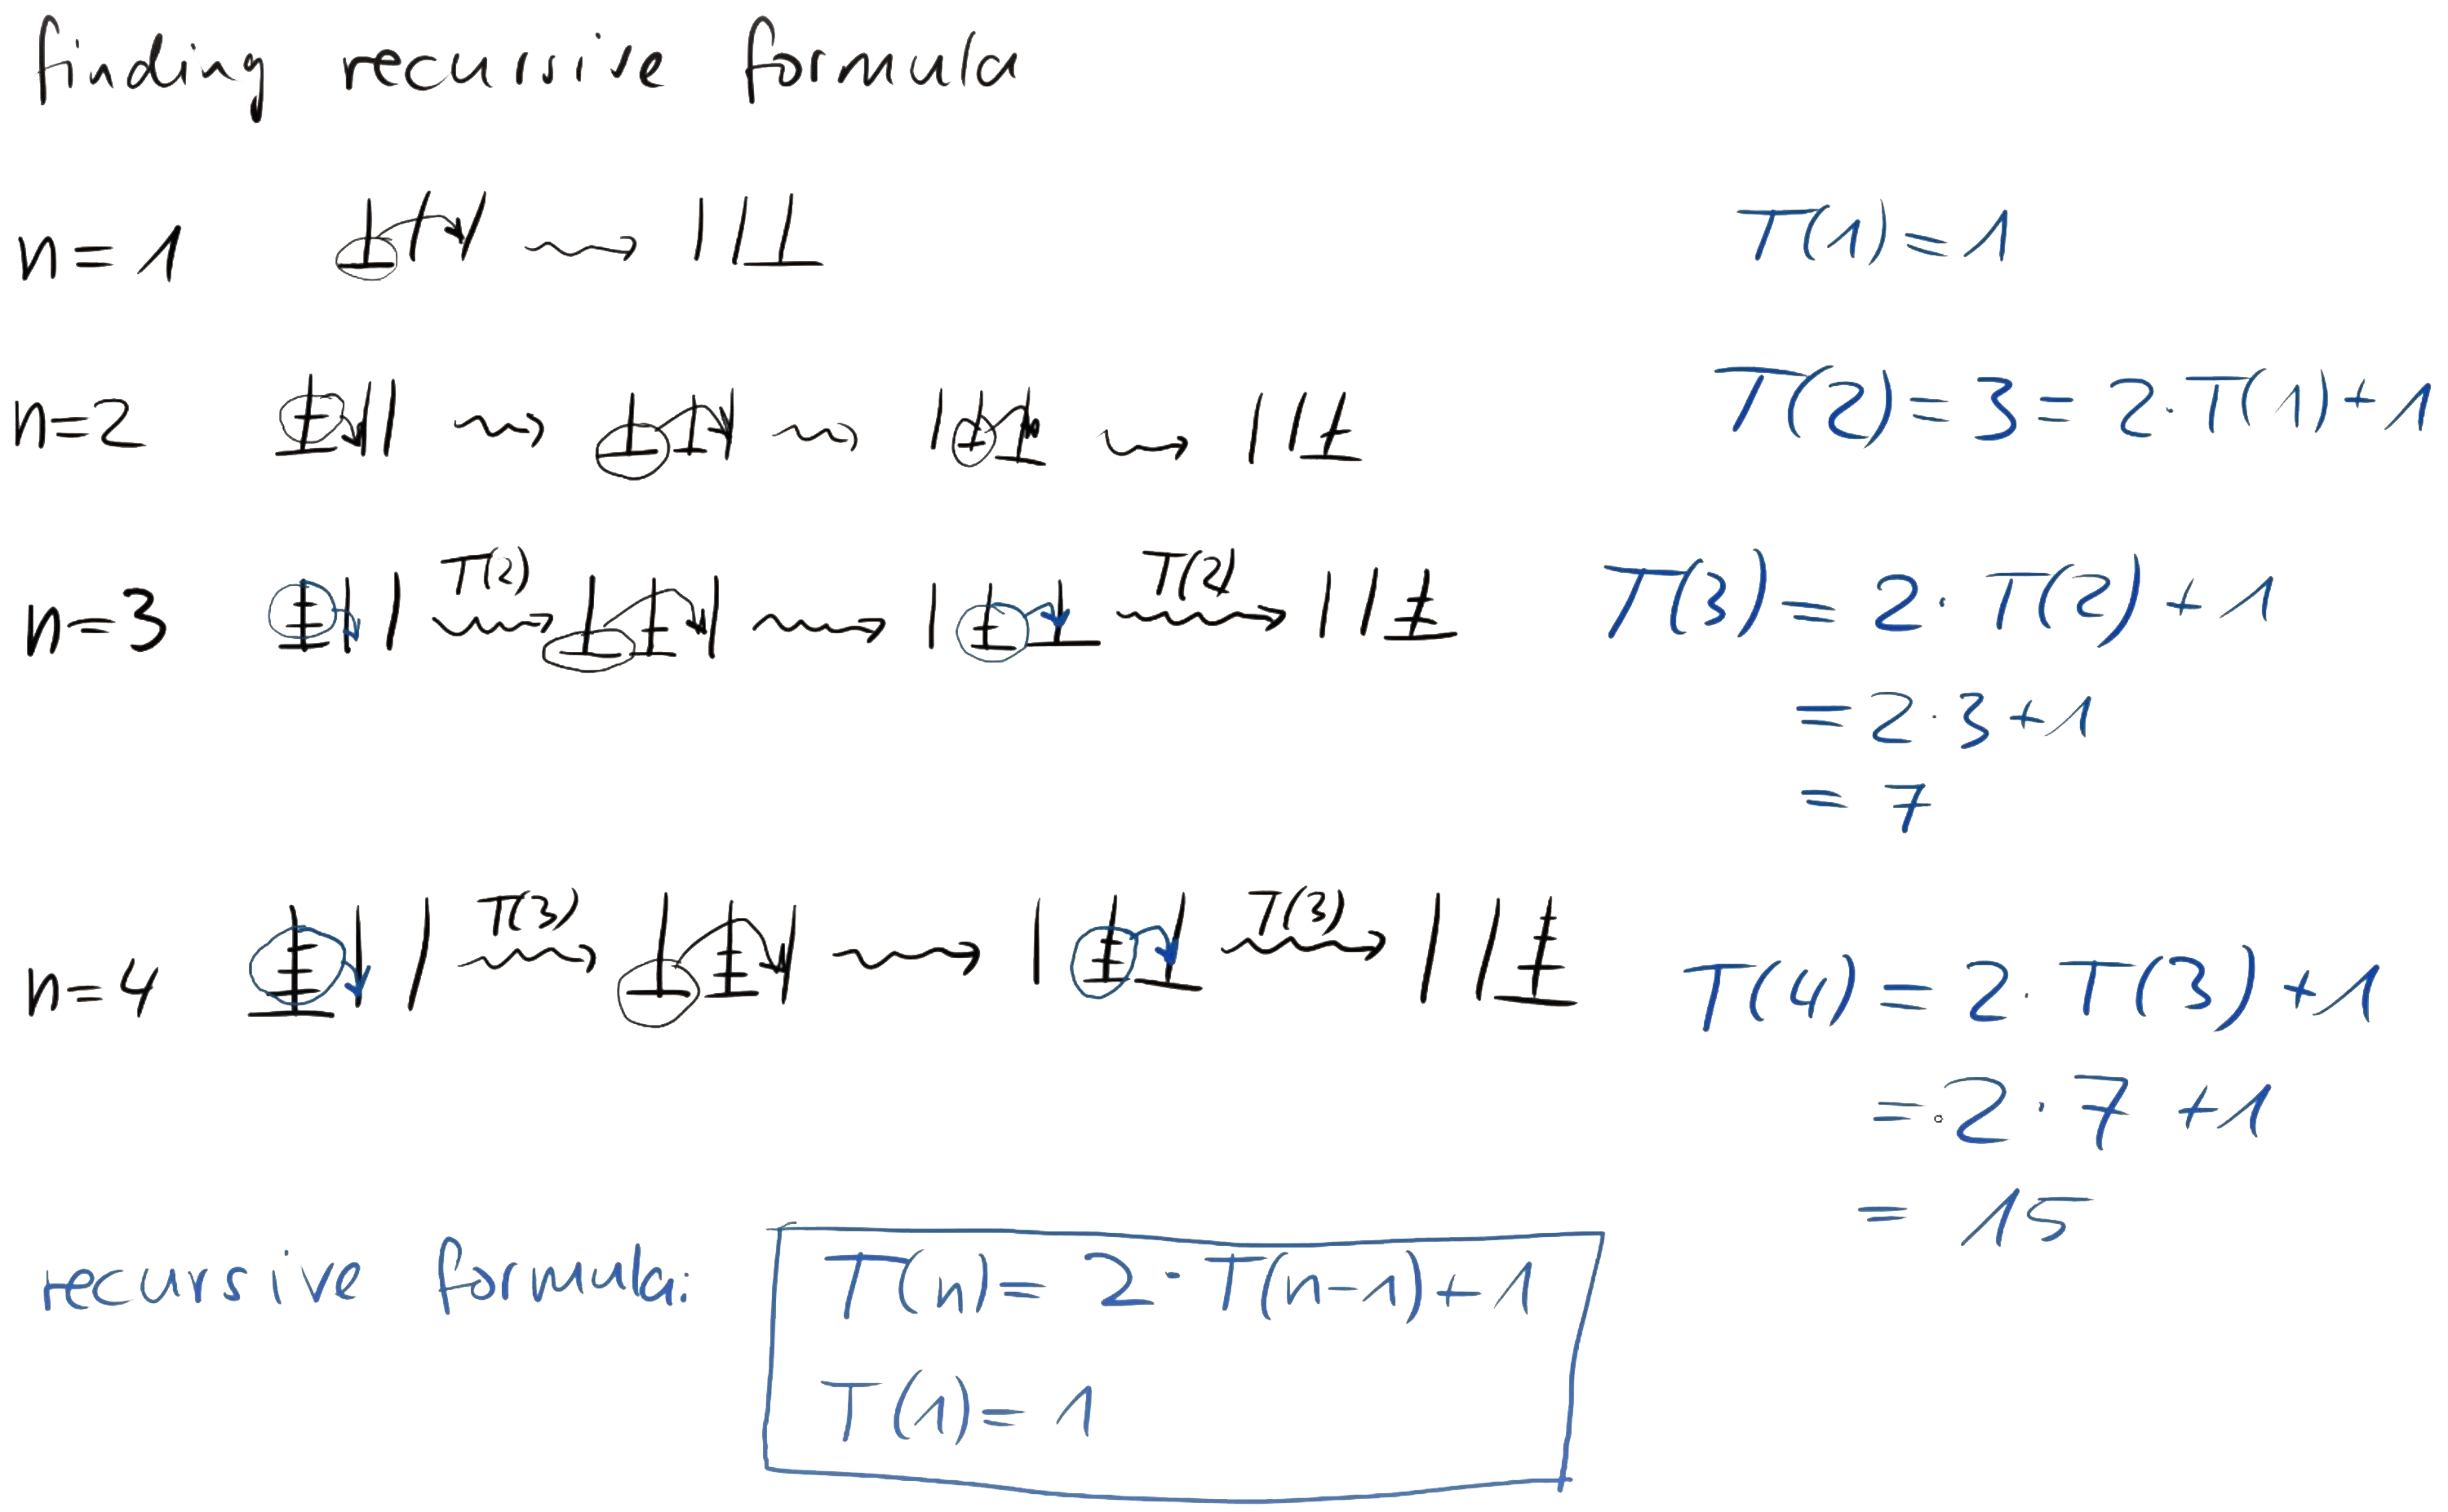
\includegraphics[width=0.7\textwidth]{figures/Tower of Hanoi.jpg}
   \label{fig:Tower of Hanoi}
\end{figure}

\pagebreak
\subsection*{Closed Form}

\vspace{1em}
\begin{minipage}{0.45\textwidth}
From the recurrence relation of TOH,
\vspace{0.5em}

$\begin{aligned}
T_n &= 2T_{(n-1)} + 1 \\
   &= 2\left(2T_{(n-2)} + 1\right) + 1 \\
   &= 2^2 T_{(n-2)} + 2 + 1 \\
   &= 2^2 \left(2T_{(n-3)} + 1\right) + 2 + 1 \\
   &= 2^3 T_{n-3} + 2^2 + 2 + 1 \\
   &\ \vdots \\
   &= 2^n T_{n-n} + \left(2^{n-1} + 2^{n-2} + \cdots + 2^1 + 2^0\right) \\
   &= 0 + \sum_{k=0}^{n-1} 2^k\\
    &= 2^{(n-1)+1} - 1  \qquad \left[\because  \sum_{k=0}^{n} 2^k = 2^{n+1} -1\right]\\
   \therefore T_n &= 2^n - 1\\
\end{aligned}$
\end{minipage}%
\hfill{\color{lightgray}\vrule}\hfill
\begin{minipage}{0.45\textwidth}
From the recurrence relation of DTOH,
\vspace{0.5em}

$\begin{aligned}
T_n &= 2T_{(n-1)} + \rgbR{2} \\
   &= 2\left(2T_{(n-2)} + 2\right) + \rgbR{2} \\
   &= 2^2 T_{(n-2)} + 2 \cdot \rgbR{2} + \rgbR{2} \\
   &= 2^2 \left(2T_{(n-3)} + 2\right) + 2 \cdot \rgbR{2} + \rgbR{2} \\
   &= 2^3 T_{n-3} + 2^2 \cdot \rgbR{2} + 2^1 \cdot \rgbR{2} + 2^0 \cdot \rgbR{2} \\
   &= 2^3 T_{n-3} + \rgbR{2}\left(2^2 + 2^1 + 2^0\right) \\
   &\ \vdots \\
   &= 2^n T_{n-n} + \rgbR{2}\left(2^{n-1} + 2^{n-2} + \cdots + 2^1 + 2^0\right) \\
   &= 0 + \rgbR{2}\sum_{k=0}^{n-1} 2^k\\
   &= \rgbR{2}\left(2^{(n-1)+1} - 1\right)\\
   \therefore T_n &= \rgbR{2}\left(2^n - 1\right)\\
\end{aligned}$
\end{minipage}

% \begin{tcolorbox}[colback=rgbB!25, boxrule=0pt, arc=4pt]
%    \centering
%    The closed-form solution for the \\ToH recurrence is:\\[0.5em]
%    $T(n) = 2^n - 1$
% \end{tcolorbox}


\vspace{2em}
\subsection*{Proof by Induction}

\vspace{1em}
\begin{minipage}[t]{0.45\textwidth}
\vspace{0pt} 
Close form proof of TOH: \ $T_n = \left(2^n - 1\right)$,

% We will prove by mathematical induction that the closed-form solution for the Tower of Hanoi recurrence is correct:
% $T(n) = 2^n - 1$
% where $T_1 = 1$ and $T_n = 2^n - 1$ for $n > 1$.
\vspace{0.5em}
\textbf{Base Case:}\\[0.5em]
For the lowest value of $n = 1$,\\[0.5em]
$T_1 = 2^1 - 1 \quad = 2 - 1 = 1$

% So, the formula holds for $n = 1$.
\vspace{1em}
\textbf{Hypothesis:}\\[0.5em]
Assume the formula holds for $n = 1$ to $k-1$,\\[0.5em]
$T_{k-1} = 2^{k-1} - 1$

\vspace{1em}
\textbf{Inductive Step:}\\[0.5em]
% We need to show it holds for $n = k$.
From the recurrence,\\[0.5em]
$\begin{aligned}
   T_k & = 2\ul[rgbRF]{T_{(k-1)}} + 1 \\
   &= 2\ul[rgbRF]{(2^{k-1} - 1)} + 1 \\
   &= 2^{k-1+1} - 2 + 1 \\
   &= 2^k - 1
\end{aligned}$

\vspace{1em}
Thus, the formula also holds for $n = k$. (Proved)
\end{minipage}%
\hfill{\color{lightgray}\vrule}\hfill
\begin{minipage}[t]{0.45\textwidth}
   \vspace{0pt} 
   Close form proof of DTOH: \ $T_n = 2 \left(2^n - 1\right)$,

   \vspace{0.5em}
   \textbf{Base Case:}\\[0.5em]
   For the lowest value of $n = 1$,\\[0.5em]
   $T_1 = 2(2^1 - 1) \quad = 2(2 - 1) = 2$
   
   \vspace{1em}
   \textbf{Hypothesis:}\\[0.5em]
   Assume the formula holds for $n = 1$ to $k-1$,\\[0.5em]
   $T_{k-1} = 2(2^{k-1} - 1)$
   
   \vspace{1em}
   \textbf{Inductive Step:}\\[0.5em]
   From the recurrence,\\[0.5em]
   $\begin{aligned}
      T_k & = 2\ul[rgbRF]{T_{(k-1)}} + 2 \\
      &= 2 \cdot \ul[rgbRF]{2(2^{k-1} - 1)} + 2 \\
      &= 2 \left[2(2^{k-1} - 1) + 1\right] \\
      &= 2 \left[2^{k-1+1} - 2 + 1\right] \\
      &= 2 \left(2^k - 2\right)
   \end{aligned}$
   
   \vspace{1em}
   Thus, the formula also holds for $n = k$. (Proved)
\end{minipage}


% \textbf{Conclusion:} By the principle of mathematical induction, the closed-form $T(n) = 2^n - 1$ is valid for all $n \geq 1$.

\pagebreak
\section{Lines in the plane}
\begin{center}
   \begin{tabular}{ccc|cccc}
      \multicolumn{2}{c}{\textbf{Rules:}}
      &&& \multicolumn{3}{c}{\textbf{Regions}}\\[1em]
      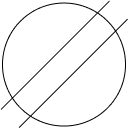
\includegraphics[width=2cm]{figures/Lines in planes/Rule-1.png}
      & 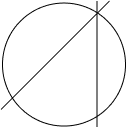
\includegraphics[width=2cm]{figures/Lines in planes/Rule-2.png}
      & \hspace{1cm}
      & \hspace{1cm}
      & 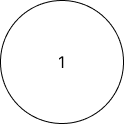
\includegraphics[width=2cm]{figures/Lines in planes/L1.png}
      & 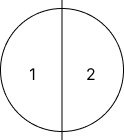
\includegraphics[width=2cm]{figures/Lines in planes/L2.png}
      & 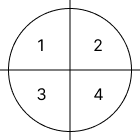
\includegraphics[width=2cm]{figures/Lines in planes/L4.png}
      \\
      \makecell{Lines can't be\\parallel to each other}
      & \makecell{Lines can't\\intersect in border}
      &&
      & $L_0 = 1$
      & $L_1 = 2$
      & $L_2 = 4$
   \end{tabular}

   \vspace{1em}
   $\therefore$ Recursive formula: $L_n = L_{n-1}+n$
\end{center}


\subsection*{Close Form}
\vspace{0.5em}
$\begin{aligned}
L_{\rgbR{n}} & =L_{\rgbR{n-1}}+\rgbR{n} \\
&= L_{n-2}+(n-1)+n \qquad\qquad\qquad\qquad
& [\because L_{\rgbR{n-1}} = L_{n-\rgbR{2}} + (\rgbR{n-1})]\\
&= L_{n-3}+(n-2)+(n-1)+n
& [\because L_{\rgbR{n-2}} = L_{n-\rgbR{3}} + (\rgbR{n-2})]\\
&\ \vdots \\
&= L_{n-n}+\cdots+(n-2)+(n-1)+n \\
&= \rgbR{L_0} + \sum_{k=1}^{n} k \\[0.5em]
&= \rgbR{1} + \frac{n(n+1)}{2}
\end{aligned}$


\subsection*{Proof by Induction}

\vspace{1em}
Proof that $n$ lines will divide a plane into \ $L_n = 1 + \frac{n(n+1)}{2}$ regions,

\vspace{0.5em}
\textbf{Base Case:}\\[0.5em]
For the lowest value of $n = 0$,\\[1em]
$L_0 = 1 + \frac{0(0+1)}{2} \quad = 1 + 0 = 1$

\vspace{1em}
\textbf{Hypothesis:}\\[0.5em]
Assume the formula holds for $n = 1$ to $n-1$,\\[1em]
$L_{n-1} = 1 + \frac{{(n-1)}({n-1}+1)}{2}
\quad = 1 + \frac{n(n-1)}{2}$

\vspace{1em}
\textbf{Inductive Step:}\\[0.5em]
From the recurrence,\\[0.5em]
$\begin{aligned}
   L_n & = \ul[rgbRF]{L_{n-1}} + n
   \ \ = \ul[rgbRF]{1 + \frac{n(n-1)}{2}} + n \\
   & = 1 + \frac{n^2-n}{2} + n
   \ \ = 1 + \frac{n^2-n+2n}{2}\\
   & = 1 + \frac{n^2+n}{2}
   \ \ = 1 + \frac{n(n+1)}{2} \\
\end{aligned}$

\vspace{1em}
Thus, the formula also holds for $n$. (Proved)


\section{Josephus Problem}

\begin{tabular}{@{}llll}
   Recurrence formula
   & $J(2n)$   & : $2J(n)-1$ & (even)\\
   & $J(2n+1)$ & : $2J(n)+1$ & (odd)
\end{tabular}

Josephus Close Form: $n = 2^m+l$ \quad and \quad $n_{th} = 2l+1$

\vspace{2em}
\begin{tabular}{@{}ll}
   $J(\rgbR{n})$: gives survival position $\to 2l+1$\\
   $\rgbR{n}$: indicates $n$ number of persons participated $\to 2^m+l$\\
\end{tabular}

\vspace{2em}
\begin{tabular}{@{}ll}
   $J(\rgbR{n})$ &$\to$ $n$-th position survived\\
   $J(\rgbR{2^m+l})$ &$\to$ $(2l+1)$-th position survived\\
\end{tabular}



\vspace{2em}
\textbf{Question:} Find $J$(103)

\textbf{Solution:} 
\textbf{Using recursion / recurrence formula:}
\begin{center}
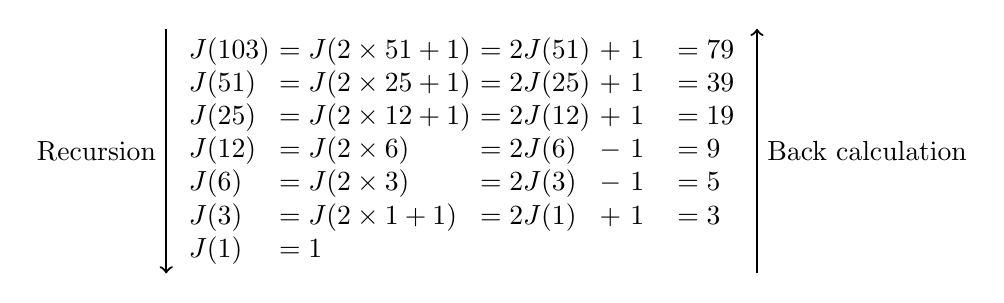
\begin{tikzpicture}
   \node[inner sep=2pt] (t) {
\begin{tabular}{l@{}l@{}l@{}ll}
$J(103)$ \ & $= J(2 \times 51 +1)$ \ & $= 2J(51)$ \ & $+ \ 1$ & $= 79$ \\
$J(51) $ & $= J(2 \times 25 +1)$ & $= 2J(25)$ \ & $+ \ 1$ & $= 39$ \\
$J(25) $ & $= J(2 \times 12 +1)$ & $= 2J(12)$ \ & $+ \ 1$ & $= 19$ \\
$J(12) $ & $= J(2 \times 6)$ & $= 2J(6)$ \ & $- \ 1$ & $= 9 $ \\
$J(6) $ & $= J(2 \times 3)$ & $= 2J(3)$ \ & $- \ 1$ & $= 5$ \\
$J(3) $ & $= J(2 \times 1 + 1)$ & $= 2J(1)$ \ & $+ \ 1$ & $= 3$ \\
$J(1) $ & $= 1$ \\
\end{tabular}
   };
   
   \draw[<-, thick] (t.south west) -- (t.north west) node[midway,left] {Recursion};
   \draw[->, thick] (t.south east) -- (t.north east) node[midway,right] {Back calculation};
\end{tikzpicture}
\end{center}


\vspace{2em}
\textbf{Using close form formula:}

Here, ${103} = {2}^{6}+{39}$,
\quad $\therefore l = 39$\\[0.5em]
\quad $\therefore$ Survival position: $n = 2l+1 = 2(39)+1 = 79$


\vspace{2em}
\textbf{Using binary property:}

J(103) = ?\\[1em]
$\text{(103)}_\text{10} = \text{(\rgbR{1}100111)}_\text{2}$\\[1em]
By applying binary left rotation,\\[1em]
we get: $\text{(100111\rgbR{1})}_\text{2} = \text{(79)}_\text{10}$


The Josephus Problem is a theoretical puzzle involving people standing in a circle and being eliminated in a fixed pattern until only one person remains. Find the smallest three values of N such that the person standing at the N/3-rd position survives.


\pagebreak
\subsection*{Proof by Induction}
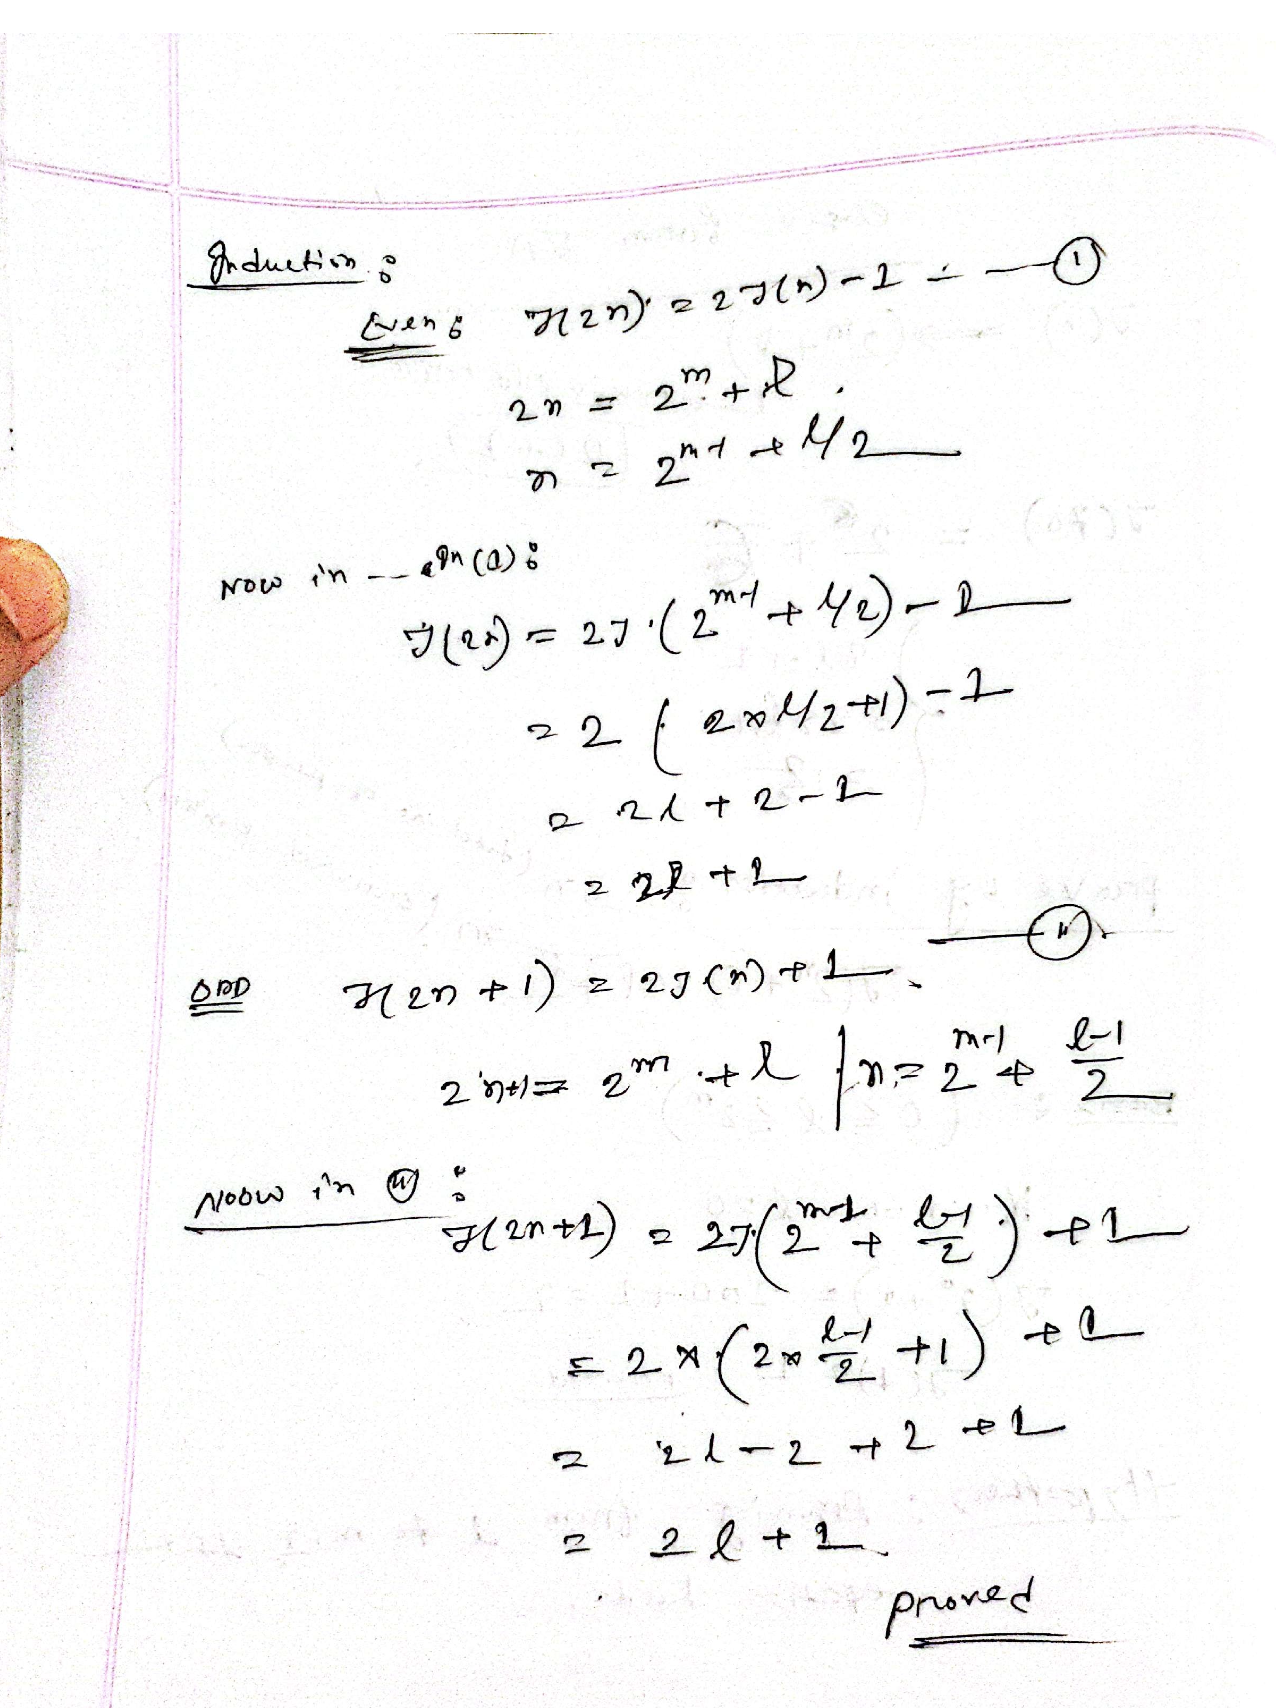
\includegraphics[width=0.9\textwidth]{figures/JInduction.png}

\pagebreak
\subsection*{Recurrence Relation}
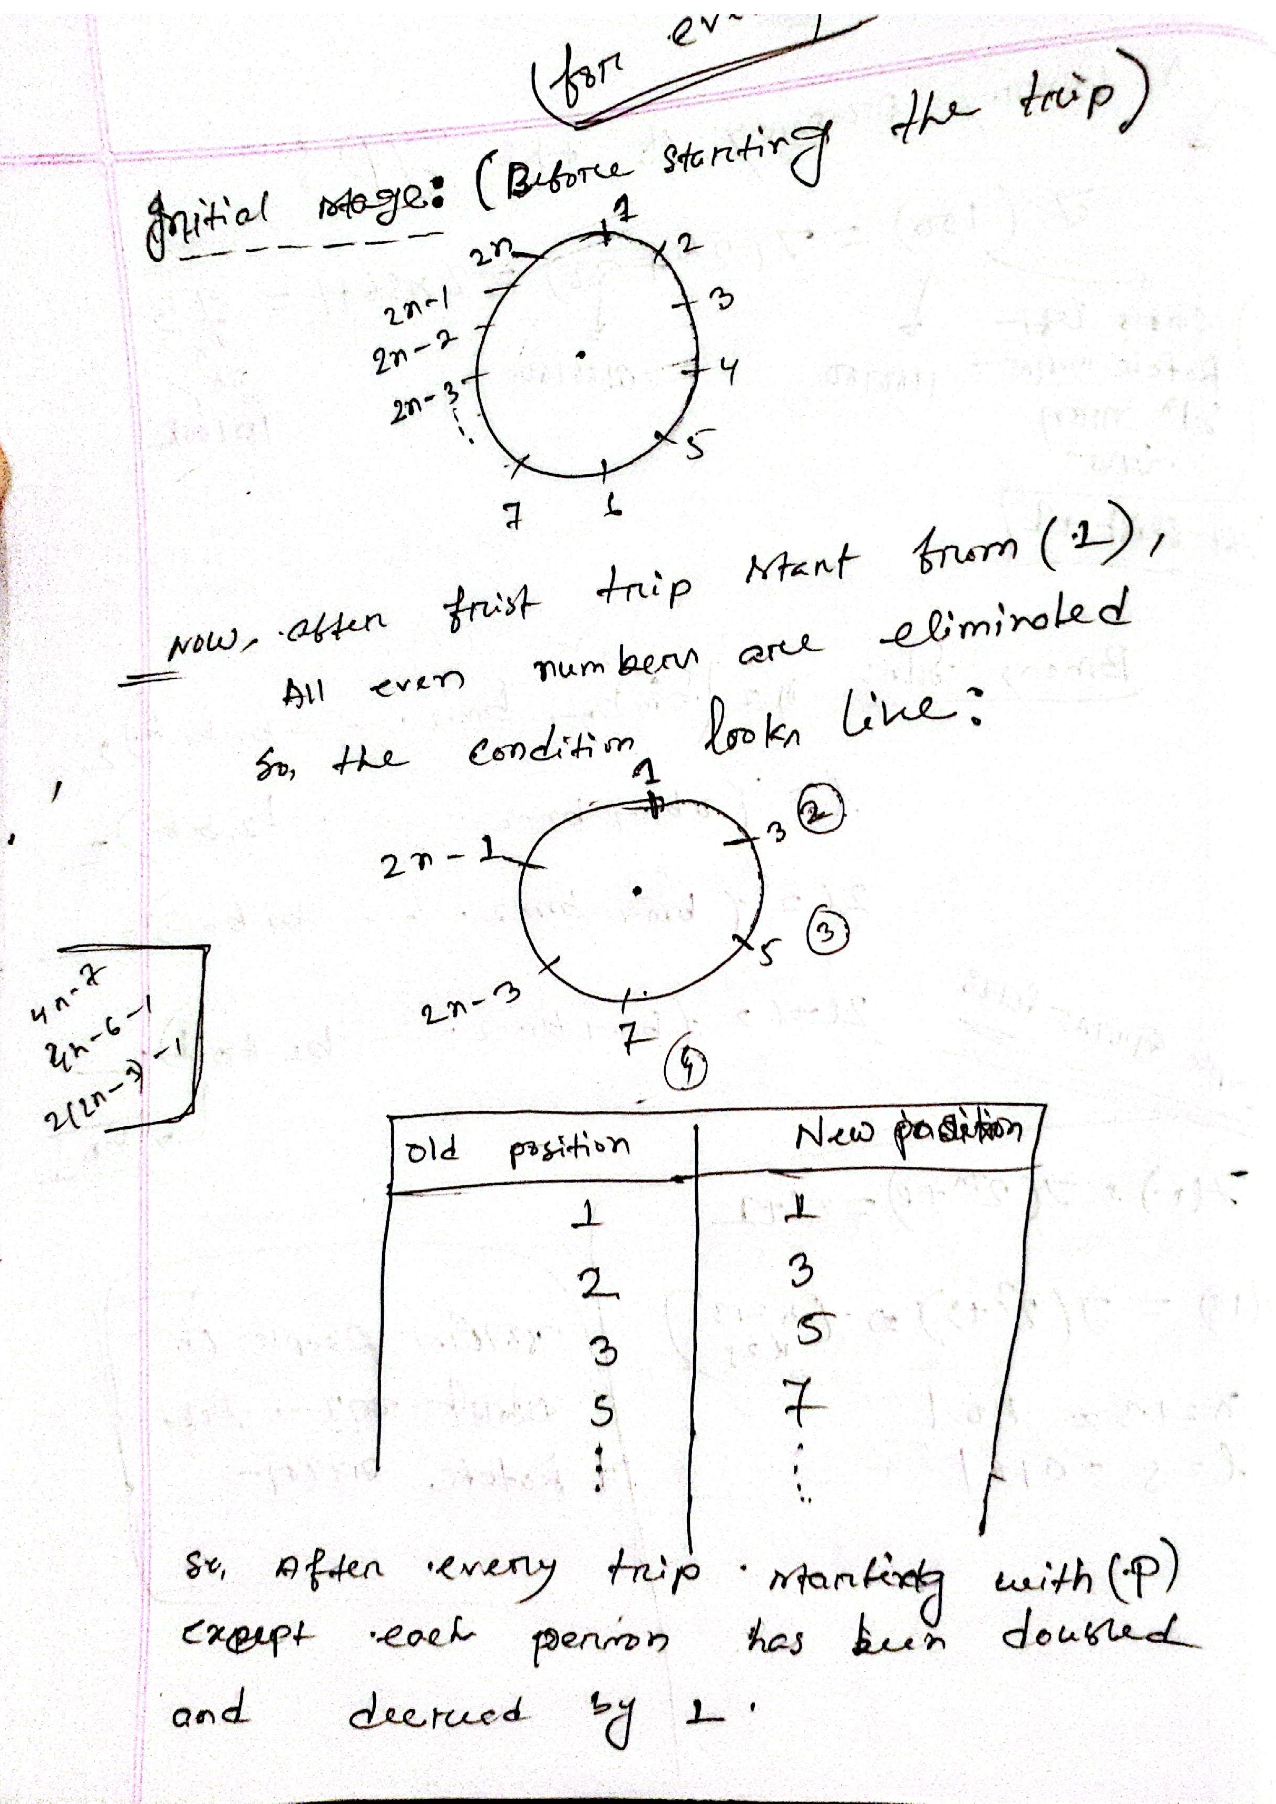
\includegraphics[width=0.9\textwidth]{figures/JR-1.png}

\pagebreak
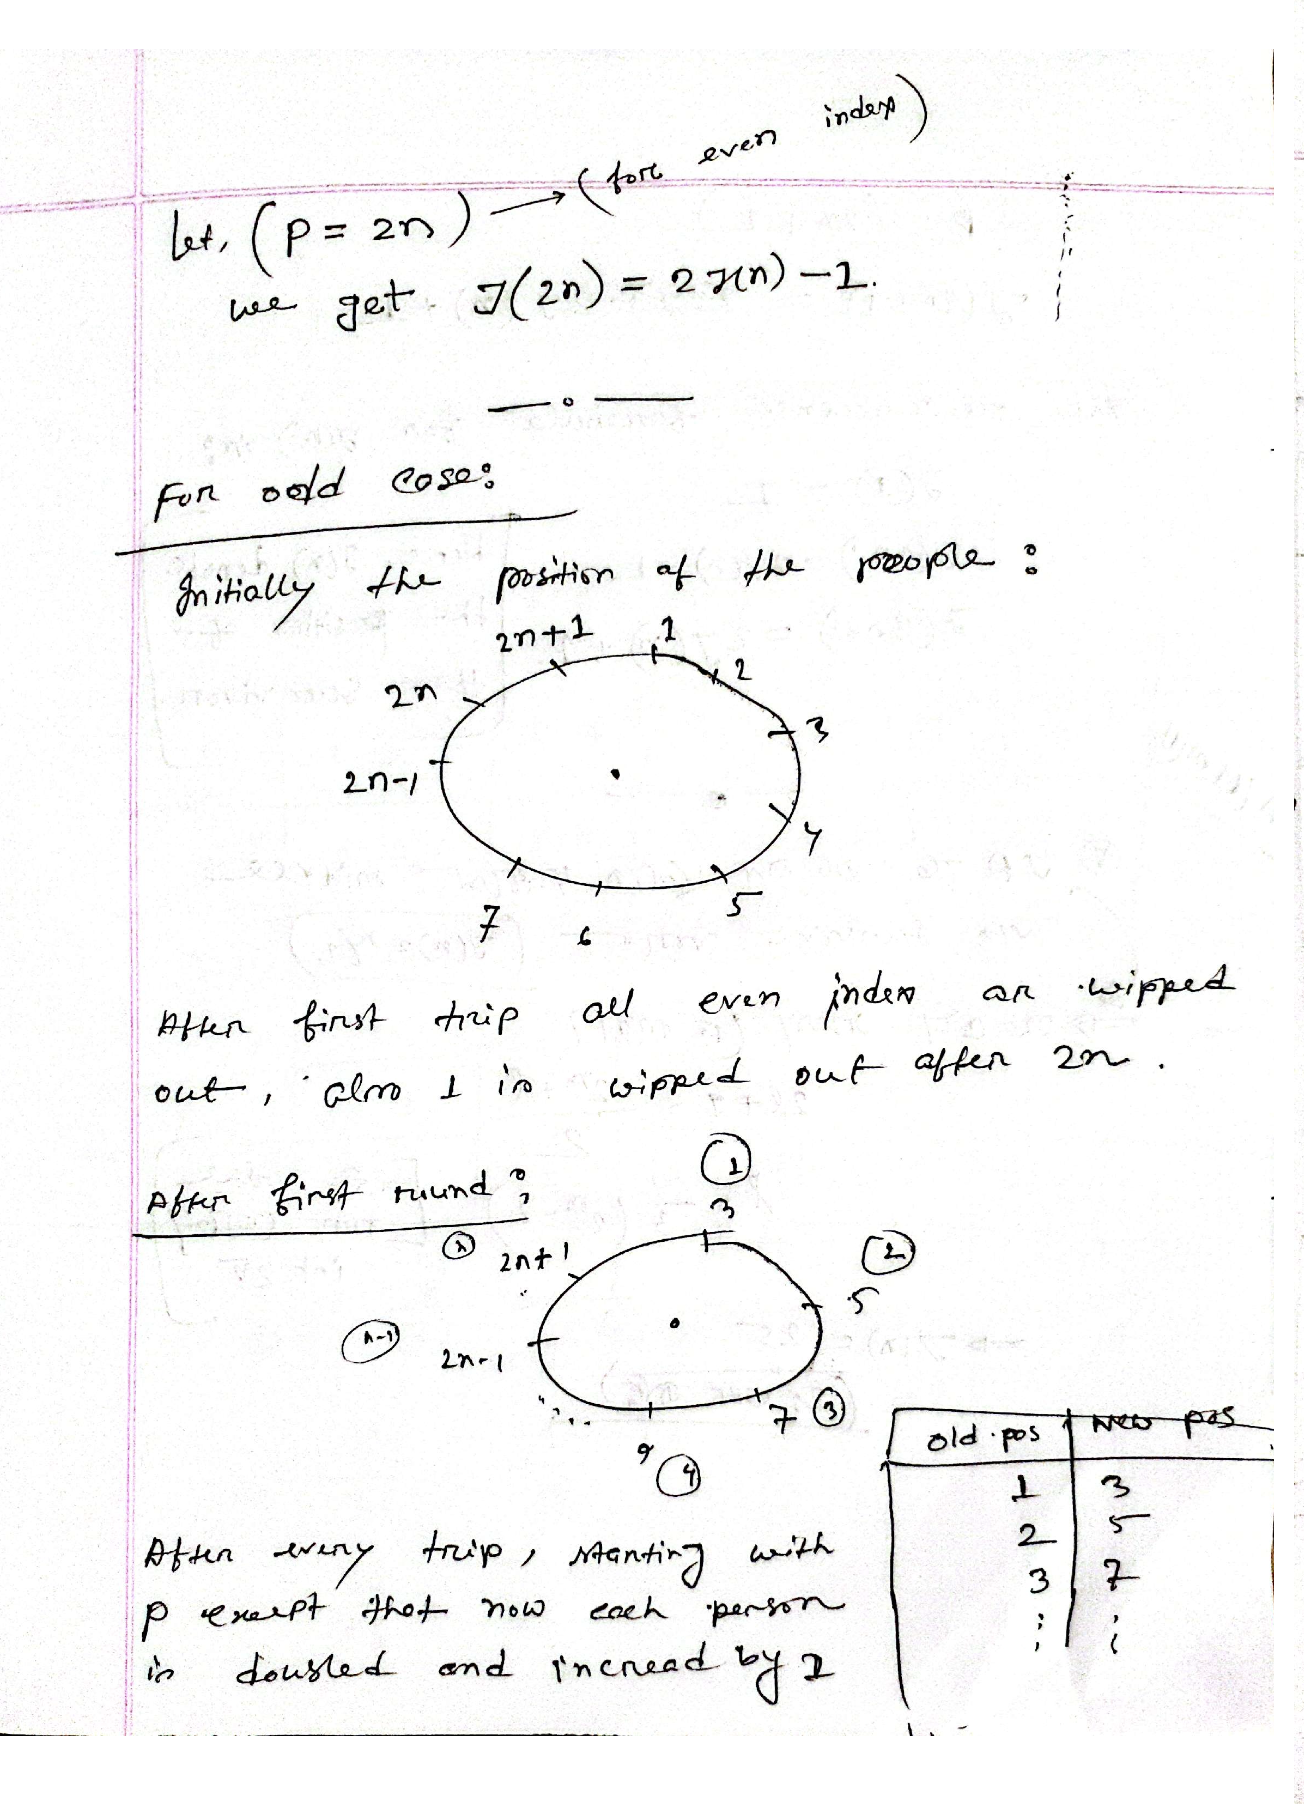
\includegraphics[width=0.9\textwidth]{figures/JR-2.png}

\pagebreak
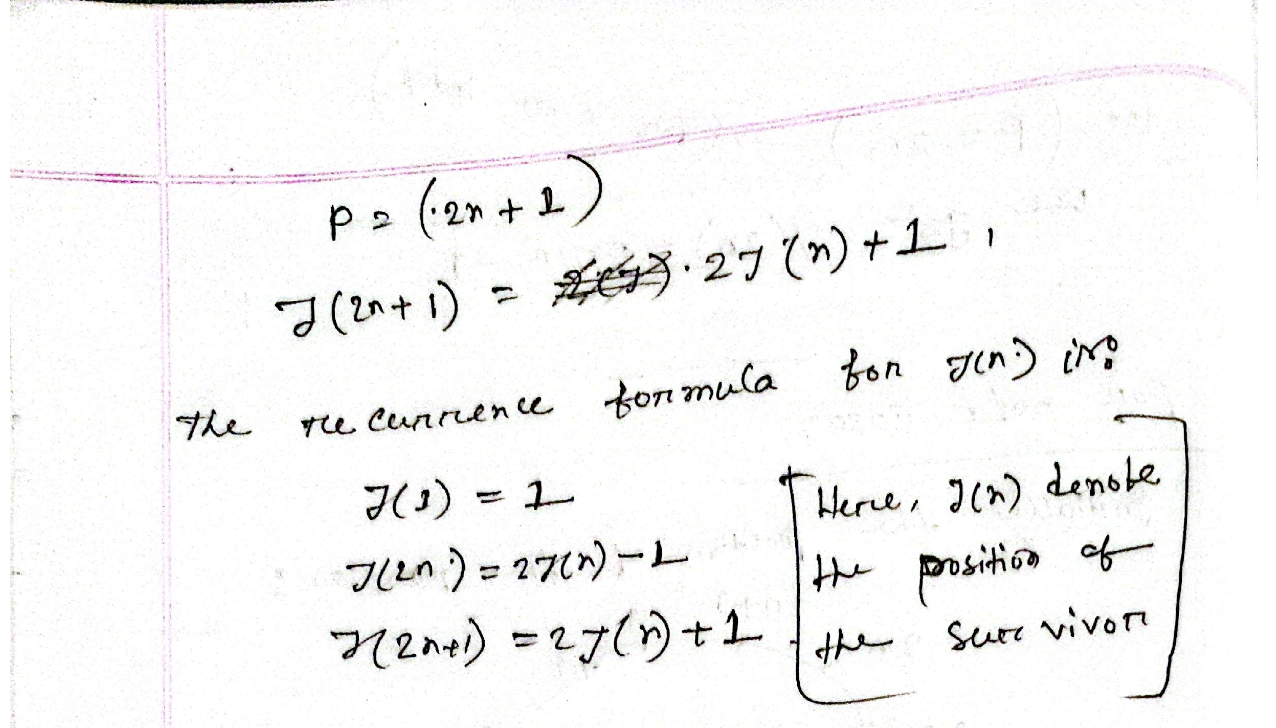
\includegraphics[width=0.9\textwidth]{figures/JR-3.png}

% \begin{tikzpicture}[scale=1.5,
%    vertex/.style={
%        circle,
%        draw=black,
%        fill=green!20,
%        minimum size=18pt,
%        inner sep=0pt
%    }
% ]

%    \def\N{13}
%    \def\R{2}
%    \pgfmathsetmacro{\angleStep}{360/\N}
   
%    \draw[very thick] (0,0) circle (\R);   
%    \foreach \i in {1,...,\N}
%    {
%        \pgfmathsetmacro{\angle}{90 - (\i-1) * \angleStep}       
%        \node[vertex] (v\i) at (\angle:\R) {\i};
%    }
% \end{tikzpicture}


\vspace{4em}
\textbf{Question:} Find the smallest 3 Values of $n$ where $n/3^\text{rd}$ person will survived.

Given,\\[1em]
$\begin{aligned}
   & J(n) =\frac{\rgbR{n}}{3} \\[1em]
   & 2l+1 =\frac{\left(\rgbR{2^m+l}\right)}{3}\\[1em]
   & 3(2l+1) = \left(\rgbR{2^m+l}\right)\\[1em]
   & 6l+3 = 2^m+l\\[1em]
   & 5l = 2^m-3\\[1em]
   & \therefore l = \frac{(2^m-3)}{5}\\[1em]
\end{aligned}$

$l$ must be an integer, so we take only those values of m where $(2m — 3)$ is divisible by 5.

Now, $\therefore m = 3, 7, 11$

\begin{tabular}{|c|c|c|c|}
   \hline $m$
   & $l = \frac{(2^m-3)}{5}$ & $n=2^m+l$ & $J(n)=2l+1 = \frac{n}{3}$ \\
   \hline 3 & 1 & 9 & 3 \\
   \hline 7 & 25 & 153 & 51 \\
   \hline 11 & 409 & 2457 & 819 \\\hline

\end{tabular}

\pagebreak
\vspace{4em}
\textbf{Question:} Find the smallest 3 Values of $n$ where $25^{th}$ person will survived.

Given,\ 
$\begin{aligned}
   J(n) = 25 \qquad
   2l+1 = 25 \qquad
   \therefore l = 12 \qquad
\end{aligned}$

\begin{tabular}{|c|c|c|l}
   \cline{1-3}
   $m$ & $l$ & $n=2^m+l$
   \\\cline{1-3}
   1 & 12 & 14 & (not accepted since 14 < 25)\\\cline{1-3}
   2 & 12 & 16 & (not accepted since 16 < 25)\\\cline{1-3}
   3 & 12 & 20 & (not accepted since 20 < 25)\\\cline{1-3}
   4 & 12 & 28 & (accepted)\\\cline{1-3}
   5 & 12 & 44 & (accepted)\\\cline{1-3}
   6 & 12 & 76 & (accepted)\\\cline{1-3}
\end{tabular}

Since 25-th person survived therefore at 25 persons needs to be participated.\\[0.5em]
Hence, $n=14,16,20$ are not acceptable.\\[0.5em]
Thus, smallest 3 values of $n=28,44,76$

\section{Ackermann Function}

% Definition: Ackermann–Péter function
\[
A(m,n) =
\begin{cases}
n+1, & m=0,\\[4pt]
A(m-1,1), & m>0,\ n=0,\\[4pt]
A(m-1,\,A(m,n-1)), & m>0,\ n>0.
\end{cases}
\]

\vspace{1em}
\textbf{Example:} Compute $A(2,2)$

\vspace{1em}
\(
\begin{aligned}
A(2,2) &= A(1,\,A(2,1)) && \ldots{(1)} \\
A(2,1) &= A(1,\,A(2,0)) && \ldots{(2)} \\
A(2,0) &= A(1,1)        && \ldots{(3)} \\
A(1,1) &= A(0,\,A(1,0)) && \ldots{(4)}
\end{aligned}
\)

From (4): $A(1,0) = A(0,1) = 2 \;\;\Rightarrow\; A(1,1) = A(0,2) = 3.$

From (3): $A(2,0) = A(1,1) = 3.$

From (2): $A(2,1) = A(1,3).$

Now, $A(1,3) = A(0,\,A(1,2)), \quad \ldots{(5)}$\\[0.5em]
From (5): $A(1,2) = A(0,\,A(1,1)) = A(0,3) = 4.$\\[0.5em]
From (5): $A(1,3) = A(0,4) = 5 \;\;\Rightarrow\; A(2,1) = 5.$

Finally, from (1): $A(2,2) = A(1,5).$

Compute $A(1,5) = A(0,\,A(1,4)), \quad A(1,4) = A(0,\,A(1,3)) = A(0,5) = 6.$

Thus $A(1,5) = A(0,6) = 7 \;\;\Rightarrow\; \boxed{A(2,2) = 7}.$